
% Default to the notebook output style

    


% Inherit from the specified cell style.




    
\documentclass[11pt]{article}

    
    
    \usepackage[T1]{fontenc}
    % Nicer default font (+ math font) than Computer Modern for most use cases
    \usepackage{mathpazo}

    % Basic figure setup, for now with no caption control since it's done
    % automatically by Pandoc (which extracts ![](path) syntax from Markdown).
    \usepackage{graphicx}
    % We will generate all images so they have a width \maxwidth. This means
    % that they will get their normal width if they fit onto the page, but
    % are scaled down if they would overflow the margins.
    \makeatletter
    \def\maxwidth{\ifdim\Gin@nat@width>\linewidth\linewidth
    \else\Gin@nat@width\fi}
    \makeatother
    \let\Oldincludegraphics\includegraphics
    % Set max figure width to be 80% of text width, for now hardcoded.
    \renewcommand{\includegraphics}[1]{\Oldincludegraphics[width=.8\maxwidth]{#1}}
    % Ensure that by default, figures have no caption (until we provide a
    % proper Figure object with a Caption API and a way to capture that
    % in the conversion process - todo).
    \usepackage{caption}
    \DeclareCaptionLabelFormat{nolabel}{}
    \captionsetup{labelformat=nolabel}

    \usepackage{adjustbox} % Used to constrain images to a maximum size 
    \usepackage{xcolor} % Allow colors to be defined
    \usepackage{enumerate} % Needed for markdown enumerations to work
    \usepackage{geometry} % Used to adjust the document margins
    \usepackage{amsmath} % Equations
    \usepackage{amssymb} % Equations
    \usepackage{textcomp} % defines textquotesingle
    % Hack from http://tex.stackexchange.com/a/47451/13684:
    \AtBeginDocument{%
        \def\PYZsq{\textquotesingle}% Upright quotes in Pygmentized code
    }
    \usepackage{upquote} % Upright quotes for verbatim code
    \usepackage{eurosym} % defines \euro
    \usepackage[mathletters]{ucs} % Extended unicode (utf-8) support
    \usepackage[utf8x]{inputenc} % Allow utf-8 characters in the tex document
    \usepackage{fancyvrb} % verbatim replacement that allows latex
    \usepackage{grffile} % extends the file name processing of package graphics 
                         % to support a larger range 
    % The hyperref package gives us a pdf with properly built
    % internal navigation ('pdf bookmarks' for the table of contents,
    % internal cross-reference links, web links for URLs, etc.)
    \usepackage{hyperref}
    \usepackage{longtable} % longtable support required by pandoc >1.10
    \usepackage{booktabs}  % table support for pandoc > 1.12.2
    \usepackage[inline]{enumitem} % IRkernel/repr support (it uses the enumerate* environment)
    \usepackage[normalem]{ulem} % ulem is needed to support strikethroughs (\sout)
                                % normalem makes italics be italics, not underlines
    

    
    
    % Colors for the hyperref package
    \definecolor{urlcolor}{rgb}{0,.145,.698}
    \definecolor{linkcolor}{rgb}{.71,0.21,0.01}
    \definecolor{citecolor}{rgb}{.12,.54,.11}

    % ANSI colors
    \definecolor{ansi-black}{HTML}{3E424D}
    \definecolor{ansi-black-intense}{HTML}{282C36}
    \definecolor{ansi-red}{HTML}{E75C58}
    \definecolor{ansi-red-intense}{HTML}{B22B31}
    \definecolor{ansi-green}{HTML}{00A250}
    \definecolor{ansi-green-intense}{HTML}{007427}
    \definecolor{ansi-yellow}{HTML}{DDB62B}
    \definecolor{ansi-yellow-intense}{HTML}{B27D12}
    \definecolor{ansi-blue}{HTML}{208FFB}
    \definecolor{ansi-blue-intense}{HTML}{0065CA}
    \definecolor{ansi-magenta}{HTML}{D160C4}
    \definecolor{ansi-magenta-intense}{HTML}{A03196}
    \definecolor{ansi-cyan}{HTML}{60C6C8}
    \definecolor{ansi-cyan-intense}{HTML}{258F8F}
    \definecolor{ansi-white}{HTML}{C5C1B4}
    \definecolor{ansi-white-intense}{HTML}{A1A6B2}

    % commands and environments needed by pandoc snippets
    % extracted from the output of `pandoc -s`
    \providecommand{\tightlist}{%
      \setlength{\itemsep}{0pt}\setlength{\parskip}{0pt}}
    \DefineVerbatimEnvironment{Highlighting}{Verbatim}{commandchars=\\\{\}}
    % Add ',fontsize=\small' for more characters per line
    \newenvironment{Shaded}{}{}
    \newcommand{\KeywordTok}[1]{\textcolor[rgb]{0.00,0.44,0.13}{\textbf{{#1}}}}
    \newcommand{\DataTypeTok}[1]{\textcolor[rgb]{0.56,0.13,0.00}{{#1}}}
    \newcommand{\DecValTok}[1]{\textcolor[rgb]{0.25,0.63,0.44}{{#1}}}
    \newcommand{\BaseNTok}[1]{\textcolor[rgb]{0.25,0.63,0.44}{{#1}}}
    \newcommand{\FloatTok}[1]{\textcolor[rgb]{0.25,0.63,0.44}{{#1}}}
    \newcommand{\CharTok}[1]{\textcolor[rgb]{0.25,0.44,0.63}{{#1}}}
    \newcommand{\StringTok}[1]{\textcolor[rgb]{0.25,0.44,0.63}{{#1}}}
    \newcommand{\CommentTok}[1]{\textcolor[rgb]{0.38,0.63,0.69}{\textit{{#1}}}}
    \newcommand{\OtherTok}[1]{\textcolor[rgb]{0.00,0.44,0.13}{{#1}}}
    \newcommand{\AlertTok}[1]{\textcolor[rgb]{1.00,0.00,0.00}{\textbf{{#1}}}}
    \newcommand{\FunctionTok}[1]{\textcolor[rgb]{0.02,0.16,0.49}{{#1}}}
    \newcommand{\RegionMarkerTok}[1]{{#1}}
    \newcommand{\ErrorTok}[1]{\textcolor[rgb]{1.00,0.00,0.00}{\textbf{{#1}}}}
    \newcommand{\NormalTok}[1]{{#1}}
    
    % Additional commands for more recent versions of Pandoc
    \newcommand{\ConstantTok}[1]{\textcolor[rgb]{0.53,0.00,0.00}{{#1}}}
    \newcommand{\SpecialCharTok}[1]{\textcolor[rgb]{0.25,0.44,0.63}{{#1}}}
    \newcommand{\VerbatimStringTok}[1]{\textcolor[rgb]{0.25,0.44,0.63}{{#1}}}
    \newcommand{\SpecialStringTok}[1]{\textcolor[rgb]{0.73,0.40,0.53}{{#1}}}
    \newcommand{\ImportTok}[1]{{#1}}
    \newcommand{\DocumentationTok}[1]{\textcolor[rgb]{0.73,0.13,0.13}{\textit{{#1}}}}
    \newcommand{\AnnotationTok}[1]{\textcolor[rgb]{0.38,0.63,0.69}{\textbf{\textit{{#1}}}}}
    \newcommand{\CommentVarTok}[1]{\textcolor[rgb]{0.38,0.63,0.69}{\textbf{\textit{{#1}}}}}
    \newcommand{\VariableTok}[1]{\textcolor[rgb]{0.10,0.09,0.49}{{#1}}}
    \newcommand{\ControlFlowTok}[1]{\textcolor[rgb]{0.00,0.44,0.13}{\textbf{{#1}}}}
    \newcommand{\OperatorTok}[1]{\textcolor[rgb]{0.40,0.40,0.40}{{#1}}}
    \newcommand{\BuiltInTok}[1]{{#1}}
    \newcommand{\ExtensionTok}[1]{{#1}}
    \newcommand{\PreprocessorTok}[1]{\textcolor[rgb]{0.74,0.48,0.00}{{#1}}}
    \newcommand{\AttributeTok}[1]{\textcolor[rgb]{0.49,0.56,0.16}{{#1}}}
    \newcommand{\InformationTok}[1]{\textcolor[rgb]{0.38,0.63,0.69}{\textbf{\textit{{#1}}}}}
    \newcommand{\WarningTok}[1]{\textcolor[rgb]{0.38,0.63,0.69}{\textbf{\textit{{#1}}}}}
    
    
    % Define a nice break command that doesn't care if a line doesn't already
    % exist.
    \def\br{\hspace*{\fill} \\* }
    % Math Jax compatability definitions
    \def\gt{>}
    \def\lt{<}
    % Document parameters
    \title{temporary}
    
    
    

    % Pygments definitions
    
\makeatletter
\def\PY@reset{\let\PY@it=\relax \let\PY@bf=\relax%
    \let\PY@ul=\relax \let\PY@tc=\relax%
    \let\PY@bc=\relax \let\PY@ff=\relax}
\def\PY@tok#1{\csname PY@tok@#1\endcsname}
\def\PY@toks#1+{\ifx\relax#1\empty\else%
    \PY@tok{#1}\expandafter\PY@toks\fi}
\def\PY@do#1{\PY@bc{\PY@tc{\PY@ul{%
    \PY@it{\PY@bf{\PY@ff{#1}}}}}}}
\def\PY#1#2{\PY@reset\PY@toks#1+\relax+\PY@do{#2}}

\expandafter\def\csname PY@tok@w\endcsname{\def\PY@tc##1{\textcolor[rgb]{0.73,0.73,0.73}{##1}}}
\expandafter\def\csname PY@tok@c\endcsname{\let\PY@it=\textit\def\PY@tc##1{\textcolor[rgb]{0.25,0.50,0.50}{##1}}}
\expandafter\def\csname PY@tok@cp\endcsname{\def\PY@tc##1{\textcolor[rgb]{0.74,0.48,0.00}{##1}}}
\expandafter\def\csname PY@tok@k\endcsname{\let\PY@bf=\textbf\def\PY@tc##1{\textcolor[rgb]{0.00,0.50,0.00}{##1}}}
\expandafter\def\csname PY@tok@kp\endcsname{\def\PY@tc##1{\textcolor[rgb]{0.00,0.50,0.00}{##1}}}
\expandafter\def\csname PY@tok@kt\endcsname{\def\PY@tc##1{\textcolor[rgb]{0.69,0.00,0.25}{##1}}}
\expandafter\def\csname PY@tok@o\endcsname{\def\PY@tc##1{\textcolor[rgb]{0.40,0.40,0.40}{##1}}}
\expandafter\def\csname PY@tok@ow\endcsname{\let\PY@bf=\textbf\def\PY@tc##1{\textcolor[rgb]{0.67,0.13,1.00}{##1}}}
\expandafter\def\csname PY@tok@nb\endcsname{\def\PY@tc##1{\textcolor[rgb]{0.00,0.50,0.00}{##1}}}
\expandafter\def\csname PY@tok@nf\endcsname{\def\PY@tc##1{\textcolor[rgb]{0.00,0.00,1.00}{##1}}}
\expandafter\def\csname PY@tok@nc\endcsname{\let\PY@bf=\textbf\def\PY@tc##1{\textcolor[rgb]{0.00,0.00,1.00}{##1}}}
\expandafter\def\csname PY@tok@nn\endcsname{\let\PY@bf=\textbf\def\PY@tc##1{\textcolor[rgb]{0.00,0.00,1.00}{##1}}}
\expandafter\def\csname PY@tok@ne\endcsname{\let\PY@bf=\textbf\def\PY@tc##1{\textcolor[rgb]{0.82,0.25,0.23}{##1}}}
\expandafter\def\csname PY@tok@nv\endcsname{\def\PY@tc##1{\textcolor[rgb]{0.10,0.09,0.49}{##1}}}
\expandafter\def\csname PY@tok@no\endcsname{\def\PY@tc##1{\textcolor[rgb]{0.53,0.00,0.00}{##1}}}
\expandafter\def\csname PY@tok@nl\endcsname{\def\PY@tc##1{\textcolor[rgb]{0.63,0.63,0.00}{##1}}}
\expandafter\def\csname PY@tok@ni\endcsname{\let\PY@bf=\textbf\def\PY@tc##1{\textcolor[rgb]{0.60,0.60,0.60}{##1}}}
\expandafter\def\csname PY@tok@na\endcsname{\def\PY@tc##1{\textcolor[rgb]{0.49,0.56,0.16}{##1}}}
\expandafter\def\csname PY@tok@nt\endcsname{\let\PY@bf=\textbf\def\PY@tc##1{\textcolor[rgb]{0.00,0.50,0.00}{##1}}}
\expandafter\def\csname PY@tok@nd\endcsname{\def\PY@tc##1{\textcolor[rgb]{0.67,0.13,1.00}{##1}}}
\expandafter\def\csname PY@tok@s\endcsname{\def\PY@tc##1{\textcolor[rgb]{0.73,0.13,0.13}{##1}}}
\expandafter\def\csname PY@tok@sd\endcsname{\let\PY@it=\textit\def\PY@tc##1{\textcolor[rgb]{0.73,0.13,0.13}{##1}}}
\expandafter\def\csname PY@tok@si\endcsname{\let\PY@bf=\textbf\def\PY@tc##1{\textcolor[rgb]{0.73,0.40,0.53}{##1}}}
\expandafter\def\csname PY@tok@se\endcsname{\let\PY@bf=\textbf\def\PY@tc##1{\textcolor[rgb]{0.73,0.40,0.13}{##1}}}
\expandafter\def\csname PY@tok@sr\endcsname{\def\PY@tc##1{\textcolor[rgb]{0.73,0.40,0.53}{##1}}}
\expandafter\def\csname PY@tok@ss\endcsname{\def\PY@tc##1{\textcolor[rgb]{0.10,0.09,0.49}{##1}}}
\expandafter\def\csname PY@tok@sx\endcsname{\def\PY@tc##1{\textcolor[rgb]{0.00,0.50,0.00}{##1}}}
\expandafter\def\csname PY@tok@m\endcsname{\def\PY@tc##1{\textcolor[rgb]{0.40,0.40,0.40}{##1}}}
\expandafter\def\csname PY@tok@gh\endcsname{\let\PY@bf=\textbf\def\PY@tc##1{\textcolor[rgb]{0.00,0.00,0.50}{##1}}}
\expandafter\def\csname PY@tok@gu\endcsname{\let\PY@bf=\textbf\def\PY@tc##1{\textcolor[rgb]{0.50,0.00,0.50}{##1}}}
\expandafter\def\csname PY@tok@gd\endcsname{\def\PY@tc##1{\textcolor[rgb]{0.63,0.00,0.00}{##1}}}
\expandafter\def\csname PY@tok@gi\endcsname{\def\PY@tc##1{\textcolor[rgb]{0.00,0.63,0.00}{##1}}}
\expandafter\def\csname PY@tok@gr\endcsname{\def\PY@tc##1{\textcolor[rgb]{1.00,0.00,0.00}{##1}}}
\expandafter\def\csname PY@tok@ge\endcsname{\let\PY@it=\textit}
\expandafter\def\csname PY@tok@gs\endcsname{\let\PY@bf=\textbf}
\expandafter\def\csname PY@tok@gp\endcsname{\let\PY@bf=\textbf\def\PY@tc##1{\textcolor[rgb]{0.00,0.00,0.50}{##1}}}
\expandafter\def\csname PY@tok@go\endcsname{\def\PY@tc##1{\textcolor[rgb]{0.53,0.53,0.53}{##1}}}
\expandafter\def\csname PY@tok@gt\endcsname{\def\PY@tc##1{\textcolor[rgb]{0.00,0.27,0.87}{##1}}}
\expandafter\def\csname PY@tok@err\endcsname{\def\PY@bc##1{\setlength{\fboxsep}{0pt}\fcolorbox[rgb]{1.00,0.00,0.00}{1,1,1}{\strut ##1}}}
\expandafter\def\csname PY@tok@kc\endcsname{\let\PY@bf=\textbf\def\PY@tc##1{\textcolor[rgb]{0.00,0.50,0.00}{##1}}}
\expandafter\def\csname PY@tok@kd\endcsname{\let\PY@bf=\textbf\def\PY@tc##1{\textcolor[rgb]{0.00,0.50,0.00}{##1}}}
\expandafter\def\csname PY@tok@kn\endcsname{\let\PY@bf=\textbf\def\PY@tc##1{\textcolor[rgb]{0.00,0.50,0.00}{##1}}}
\expandafter\def\csname PY@tok@kr\endcsname{\let\PY@bf=\textbf\def\PY@tc##1{\textcolor[rgb]{0.00,0.50,0.00}{##1}}}
\expandafter\def\csname PY@tok@bp\endcsname{\def\PY@tc##1{\textcolor[rgb]{0.00,0.50,0.00}{##1}}}
\expandafter\def\csname PY@tok@fm\endcsname{\def\PY@tc##1{\textcolor[rgb]{0.00,0.00,1.00}{##1}}}
\expandafter\def\csname PY@tok@vc\endcsname{\def\PY@tc##1{\textcolor[rgb]{0.10,0.09,0.49}{##1}}}
\expandafter\def\csname PY@tok@vg\endcsname{\def\PY@tc##1{\textcolor[rgb]{0.10,0.09,0.49}{##1}}}
\expandafter\def\csname PY@tok@vi\endcsname{\def\PY@tc##1{\textcolor[rgb]{0.10,0.09,0.49}{##1}}}
\expandafter\def\csname PY@tok@vm\endcsname{\def\PY@tc##1{\textcolor[rgb]{0.10,0.09,0.49}{##1}}}
\expandafter\def\csname PY@tok@sa\endcsname{\def\PY@tc##1{\textcolor[rgb]{0.73,0.13,0.13}{##1}}}
\expandafter\def\csname PY@tok@sb\endcsname{\def\PY@tc##1{\textcolor[rgb]{0.73,0.13,0.13}{##1}}}
\expandafter\def\csname PY@tok@sc\endcsname{\def\PY@tc##1{\textcolor[rgb]{0.73,0.13,0.13}{##1}}}
\expandafter\def\csname PY@tok@dl\endcsname{\def\PY@tc##1{\textcolor[rgb]{0.73,0.13,0.13}{##1}}}
\expandafter\def\csname PY@tok@s2\endcsname{\def\PY@tc##1{\textcolor[rgb]{0.73,0.13,0.13}{##1}}}
\expandafter\def\csname PY@tok@sh\endcsname{\def\PY@tc##1{\textcolor[rgb]{0.73,0.13,0.13}{##1}}}
\expandafter\def\csname PY@tok@s1\endcsname{\def\PY@tc##1{\textcolor[rgb]{0.73,0.13,0.13}{##1}}}
\expandafter\def\csname PY@tok@mb\endcsname{\def\PY@tc##1{\textcolor[rgb]{0.40,0.40,0.40}{##1}}}
\expandafter\def\csname PY@tok@mf\endcsname{\def\PY@tc##1{\textcolor[rgb]{0.40,0.40,0.40}{##1}}}
\expandafter\def\csname PY@tok@mh\endcsname{\def\PY@tc##1{\textcolor[rgb]{0.40,0.40,0.40}{##1}}}
\expandafter\def\csname PY@tok@mi\endcsname{\def\PY@tc##1{\textcolor[rgb]{0.40,0.40,0.40}{##1}}}
\expandafter\def\csname PY@tok@il\endcsname{\def\PY@tc##1{\textcolor[rgb]{0.40,0.40,0.40}{##1}}}
\expandafter\def\csname PY@tok@mo\endcsname{\def\PY@tc##1{\textcolor[rgb]{0.40,0.40,0.40}{##1}}}
\expandafter\def\csname PY@tok@ch\endcsname{\let\PY@it=\textit\def\PY@tc##1{\textcolor[rgb]{0.25,0.50,0.50}{##1}}}
\expandafter\def\csname PY@tok@cm\endcsname{\let\PY@it=\textit\def\PY@tc##1{\textcolor[rgb]{0.25,0.50,0.50}{##1}}}
\expandafter\def\csname PY@tok@cpf\endcsname{\let\PY@it=\textit\def\PY@tc##1{\textcolor[rgb]{0.25,0.50,0.50}{##1}}}
\expandafter\def\csname PY@tok@c1\endcsname{\let\PY@it=\textit\def\PY@tc##1{\textcolor[rgb]{0.25,0.50,0.50}{##1}}}
\expandafter\def\csname PY@tok@cs\endcsname{\let\PY@it=\textit\def\PY@tc##1{\textcolor[rgb]{0.25,0.50,0.50}{##1}}}

\def\PYZbs{\char`\\}
\def\PYZus{\char`\_}
\def\PYZob{\char`\{}
\def\PYZcb{\char`\}}
\def\PYZca{\char`\^}
\def\PYZam{\char`\&}
\def\PYZlt{\char`\<}
\def\PYZgt{\char`\>}
\def\PYZsh{\char`\#}
\def\PYZpc{\char`\%}
\def\PYZdl{\char`\$}
\def\PYZhy{\char`\-}
\def\PYZsq{\char`\'}
\def\PYZdq{\char`\"}
\def\PYZti{\char`\~}
% for compatibility with earlier versions
\def\PYZat{@}
\def\PYZlb{[}
\def\PYZrb{]}
\makeatother


    % Exact colors from NB
    \definecolor{incolor}{rgb}{0.0, 0.0, 0.5}
    \definecolor{outcolor}{rgb}{0.545, 0.0, 0.0}



    
    % Prevent overflowing lines due to hard-to-break entities
    \sloppy 
    % Setup hyperref package
    \hypersetup{
      breaklinks=true,  % so long urls are correctly broken across lines
      colorlinks=true,
      urlcolor=urlcolor,
      linkcolor=linkcolor,
      citecolor=citecolor,
      }
    % Slightly bigger margins than the latex defaults
    
    \geometry{verbose,tmargin=1in,bmargin=1in,lmargin=1in,rmargin=1in}
    
    

    \begin{document}
    
    
    \maketitle
    
    

    
    \hypertarget{hidden-markov-model-hmm}{%
\subsection{Hidden Markov Model (HMM)}\label{hidden-markov-model-hmm}}

\hypertarget{problem}{%
\subsubsection{Problem}\label{problem}}

\begin{itemize}
\tightlist
\item
  Input: vector \(x:\{x_1,x_2,...,x_n\}\in O\)
\item
  Output: vector \(y:\{y_1,y_2,...,y_d\}\in T\)
\item
  Where \(x\) is the observation and \(y\) is the hidden state
\item
  \(x,y\) is usually categorical, but can be numerical
\item
  \(x\in\mathbb R,y\in\mathbb R\)
\end{itemize}

\hypertarget{modelling}{%
\subsubsection{Modelling}\label{modelling}}

\textbf{Generative Tagging Model}\\
\((x_1,...,x_n,\ y_1,...,y_n)\in S\) \emph{(set of all observed pairs)}
\(p(x_1,...,x_n,\ y_1,...,y_n)\geq0\forall(x_1,...,x_n,\ y_1,...,y_n)\)
\(\sum_{(x_1,...,x_n,\ y_1,...,y_n)\in S}p(x_1,...,x_n,\ y_1,...,y_n)=1\)\\
\(\begin{aligned}y_1^*,...,y_n^*&=\arg\max_{y_1,...,y_n}(x_1,...,x_n,\ y_1,...,y_n)\\&=f(x_1,...,x_n)\end{aligned}\)

\(\Pr(X_1=x_1,...,X_n=x_n,\ Y_1=y_1,...,Y_n=y_n)=p(x_1,...,x_n,\ y_1,...,y_n)\)
- \(Y_0=y_0=\text{"START"}\)\\
- \(Y_{n+1}=y_{n+1}=\text{"STOP"}\)

\textbf{transition parameters}\\
\(p(x_1,...,x_n,\ y_0,y_1,...,y_{n+1})=p(y_0,...,y_{n+1})p(x_1,...,x_n\mid y_0,...,y_{n+1})\)
\(\begin{aligned}p(y_0,...,y_{n+1})&=p(y_0)p(y_1\mid y_0)p(y_2\mid y_0,y_1)...p(y_{n+1}\mid y_0,...,y_n)\\&\approx p(y_0)p(y_1\mid y_0)p(y_2\mid y_1)...p(y_{n+1}\mid y_n)\\&=p(y_1\mid y_0)...p(y_{n+1}\mid y_n)\\&=\prod_{i=1}^{n+1}p(y_i\mid y_{i-1})\end{aligned}\)\\
\emph{(This is a markov sequence, independent given current tag)}

\textbf{emission parameters}\\
\(\begin{aligned}p(x_1,...,x_n\mid y_0,...,y_{n+1})&=p(x_1\mid y_0,...,y_{n+1})p(x_2\mid x_1,\ y_0,...,y_{n+1})...p(x_n\mid x_1,...,x_{n-1},\ y_0,...,y_{n+1})\\&\approx p(x_1\mid y_1)p(x_2\mid y_2)...p(x_n\mid y_n)\\&=\prod_{i=1}^np(x_i\mid y_i)\end{aligned}\)\\
\emph{(word only depends on tag)}

\textbf{tagging model}\\
\(p(x_1,...,x_n,\ y_0,...,y_{n+1})=\prod_{i=1}^{n+1}p(y_i\mid y_{i-1})\prod_{i=1}^np(x_i\mid y_i)\)\\
\textbf{Generative Process}\\
1. Set \(y_0 = \text{START}\) and let \(i=1\)\\
2. Generate tag \(y_i\) from transition parameter
\(p(y_i\mid y_{i-1})\)\\
- If \(y_i=\text{STOP}\), terminate process and return
\(y_0,...,y_{i},x_1,...,x_{i-1}\) - Otherwise, generate \(x_i\) from
emission parameter \(p(x_i\mid y_i)\) 3. Set \(i=i+1\), repeat from Step
2

\textbf{HMM Formal Definition}\\
HMM is defined by \(<T,O,\theta>\) - \textgreater{} \(T\) is the set of
states including \(\text{START}\) and \(\text{STOP}\) -
\(\{0,1,...,\mid T\mid-1\}\) \emph{(0 is START, \textbar{}T\textbar{}-1
is STOP)} - \textgreater{} \(O\) is the set of observed symbols
\emph{(i.e.~x: words)} - \textgreater{} \(\theta=<a,b>\) are the
parameters - transition parameter: \(a_{u,v}=p(y_i=v\mid y_{i-1}=u)\) -
\(\sum_{v'=1}^{\mid T\mid-1}a_{u,v'}=1 \forall u\) - emission parameter:
\(b_u(o)=p(x=o\mid y=u)\) - \(\sum_{o\in O}b_u(o)=1 \forall u\)

\hypertarget{supervised-learning}{%
\subsubsection{Supervised Learning}\label{supervised-learning}}

\begin{itemize}
\tightlist
\item
  transition parameter:
  \(a_{u,v}=\frac{\text{Count}(u;v)}{\text{Count}(u)}\)

  \begin{itemize}
  \tightlist
  \item
    percentage of times v appears after u, given u
  \end{itemize}
\item
  emission parameter:
  \(b_u(o)=\frac{\text{Count}(u\rightarrow o)}{\text{Count}(u)}\)

  \begin{itemize}
  \tightlist
  \item
    percentage of times u emits symbol o
  \end{itemize}
\end{itemize}

\hypertarget{decoding}{%
\subsubsection{Decoding}\label{decoding}}

\(\arg\max_{y_1,...,y_n}p(y_0,...,y_{n+1}\mid x_1,...,x_n;\theta)\)

\(p(x_1,...,x_n,\ y_0,...,y_{n+1};\theta)=\prod_{i=1}^{n+1}a_{y_{i-1},y_i}\prod_{i=1}^nb_{y_i}(x_i)\)

\(\begin{aligned}\arg\max_{y_1,...,y_n}p(y_0,...,y_{n+1}\mid x_1,...,x_n;\theta)&=\arg\max_{y_1,...,y_n}\frac{p(x_1,...,x_n,\ y_0,...,y_{n+1};\theta)}{p(x_1,...,x_n;\theta)}\\&=\arg\max_{y_1,...,y_n}p(x_1,...,x_n,\ y_0,...,y_{n+1};\theta)\end{aligned}\)

\hypertarget{vertibi-algorithm}{%
\subsubsection{Vertibi Algorithm}\label{vertibi-algorithm}}

joint probability of first k tags\\
\(r(y_1,...,y_k)=\prod_{i=1}^{k}a_{y_{i-1},y_i}\prod_{i=1}^kb_{y_i}(x_i)\)

\(\begin{aligned}p(x_1,...,x_n,\ y_0,...,y_{n+1})&=r(y_1,...,y_n)\cdot a_{y_{n},y_{n+1}}\\&= r(y_1,...,y_n)\cdot a_{y_{n},\text{STOP}}\end{aligned}\)

\(\pi(k,v)=\max_{(y_1,...,y_k)\in S(k,v)}r(y_1,...,y_k)\) - \(S(k,v)\)
is the set of all sequences of length k with last tag v

\textbf{Base case}\\
\(\pi(0,u)=\left\{\begin{array}{cl}1 & \text{if }u=\text{START}\\0 & \text{otherwise}\end{array}\right.\)

\textbf{Forward recursively} \(\forall k\in\{1,...,n\}\)\\
\(\pi(k,v)\max_{u\in T}\{\pi(k-1,u)\cdot a_{u,v}\cdot b_v(x_k)\}\)

\textbf{Terminate} \(y_n\text{ to STOP}\)\\
\(\max_{y_1,...,y_n}p(x_1,...,x_n,\ y_0,...,y_{n+1})=\max_{v\in T}\{\pi(n,v)\cdot a_{v,\text{STOP}}\}\)

\textbf{Backtracking}\\
\(y_n^*=\arg\max_v\{\pi(n,v)\cdot a_{v,\text{STOP}}\}\)\\
\(y_{n-1}^*=\arg\max_u\{\pi(n-1,u)\cdot a_{u,y_n^*}\}\)\\
\emph{repeat for all y}

    \hypertarget{unsupervised-learning}{%
\subsubsection{Unsupervised Learning}\label{unsupervised-learning}}

\hypertarget{hard-em}{%
\paragraph{Hard EM}\label{hard-em}}

\textbf{E-Step}\\
observation sequence:
\(\boldsymbol x^{(i)}= (x_1^{(i)},x_2^{(i)},...,x_n^{(i)})\)\\
state sequence \emph{(viterbi)}:
\(\boldsymbol y^{(i)*}= (y_1^{(i)*},y_2^{(i)*},...,y_n^{(i)*})\)

\(\text{Count}(u;v), \text{Count}(u)\ \forall u,v\in T=\{0,1,...,N+1\}\)\\
\(\text{Count}(u\rightarrow o), \text{Count}(u)\ \forall u\in T,o\in O\)

\textbf{M-Step}\\
\(a_{u,v}=\frac{\text{Count}(u;v)}{\text{Count}(u)}\)\\
\(b_u(o)=\frac{\text{Count}(u\rightarrow o}{\text{Count}(u)}\)

\hypertarget{soft-em}{%
\paragraph{Soft EM}\label{soft-em}}

\textbf{E-Step}\\
\(\text{Count}(u;v)=\sum_{i=1}^m\sum_yp(\boldsymbol y\mid\boldsymbol x^{(i)})\text{Count}(\boldsymbol x^{(i)},\boldsymbol y,u\rightarrow v)\)
- where
\(\text{Count}(\boldsymbol x^{(i)},\boldsymbol y,u\rightarrow v)\) is
number of times a trasition from u to v occurs in tag sequence y
corresponding to observation sequence \(x^{(i)}\)

\textbf{M-Step}\\
\(a_{u,v}=\frac{\text{Count}(u;v)}{\sum_{v'}\text{Count}(u;v')}\) -
where denominator ensures \(\sum_{v'=1}^{N+1}a_{u,v'}=1\)

marginal posterior probabilities:
\(p(y_j=u,y_{j+1}=v\mid\boldsymbol x;\theta)=\sum_{\boldsymbol y:y_j=u,y_{j+1}=v}p(\boldsymbol y\mid\boldsymbol x;\theta)\)\\
\(\sum_yp(\boldsymbol y\mid\boldsymbol x^{(i)})\text{Count}(\boldsymbol x^{(i)},\boldsymbol y,u\rightarrow v)=\sum_{j=0}^np(y_j=u,y_{j+1}=v\mid\boldsymbol x^{(i)};\theta)\)\\
\(P()\)

\hypertarget{forward-backward-algorithm}{%
\subsubsection{Forward-Backward
Algorithm}\label{forward-backward-algorithm}}

For every state sequence y there is - a path through the graph
\(\text{START}, <1,y_1>,...,<n,y_n>,\text{STOP}\) - state sequence
\(\boldsymbol y=y_1,...,y_n\) has score equal to
\(p(\boldsymbol x,\boldsymbol y;\theta)\) - sum of scores for all paths
from START to state (j,u), \(\alpha_u(j)\) - sum of scores for all paths
from state (j,u) to STOP, \(\beta_u(j)\)\\
Given \(x_1,...,x_n\forall u\in 1,...,N,\ j\in1,...,n\)

\textbf{forward probability}\\
\(\alpha_u(j)=p(x_1,...,x_{j-1},y_j=u;\theta)\) - base case:
\(\alpha_u(1)=a_{\text{START},u}\forall u\in1,...,N-1\) - recursive
case:
\(\alpha_u(j+1)=\sum_v\alpha_v(j)a_{v,u}b_v(x_j)\forall u\in1,...,N-1,\ j\in1,...,n-1\)

\textbf{backward probability}\\
\(\beta_u(j)=p(x_j,...,x_n\mid y_j=u;\theta)\) - base case:
\(\beta_u(n)=a_{u,\text{STOP}}b_u(x_n)\forall u\in1,...,N-1\) -
recursive case:
\(\beta_u(j)=\sum_va_{u,v}b_u(x_j)\beta_u(j+1)\forall u\in1,...,N-1,\ j\in n-1,...,1\)

\textbf{Transition parameters}\\
\(\text{Count}(u;v)=\sum_{i=1}^m\text{Count}^{(i)}(u;v)\)\\
expected number of times we see u,v pair from ith instance\\
\(\text{Count}^{(i)}(u;v)=\sum_{j=0}^n\frac{1}{Z}\alpha_u(j)b_u(k_j^{(i)})\alpha_{u,v}\beta_u(j+1)\)\\
\(Z=\sum_{u'}\alpha_{u'}(j)\beta_{u'}(j)\)

\(\text{Count}^{(i)}(u)=\sum_{j=1}^n\frac{1}{Z}\alpha_u(j)\beta_u(j)\)\\
\(Z=\sum_{u'}\alpha_{u'}(j)\beta_{u'}(j) \forall j\in1,...,n\)

\textbf{emission parameters}\\
\(\text{Count}(u\rightarrow o)=\sum_{i=1}^m\text{Count}^{(i)}(u\rightarrow o)\)\\
\(\text{Count}^{(i)}(u\rightarrow)=\sum_{j:x_j^{(i)}=o}\frac{1}{Z}\alpha_u(j)\beta_u(j)\)\\
\(Z=\sum_{u'}\alpha_{u'}(j)\beta_{u'}(j)\)

\textbf{max marginal decoding}\\
\(\begin{aligned}y_i^*&=\arg\max_up(y_i=u\mid x_1,...,x_n;\theta)\\&=\arg\max_u\frac{\alpha_u(i)\beta_u(i)}{\sum_v\alpha_v(j)\beta_v(j)}\\&=\arg\max_u\alpha_u(i)\beta_u(i)\end{aligned}\)

    \hypertarget{reinforcement-learning}{%
\section{Reinforcement Learning}\label{reinforcement-learning}}

\begin{figure}
\centering
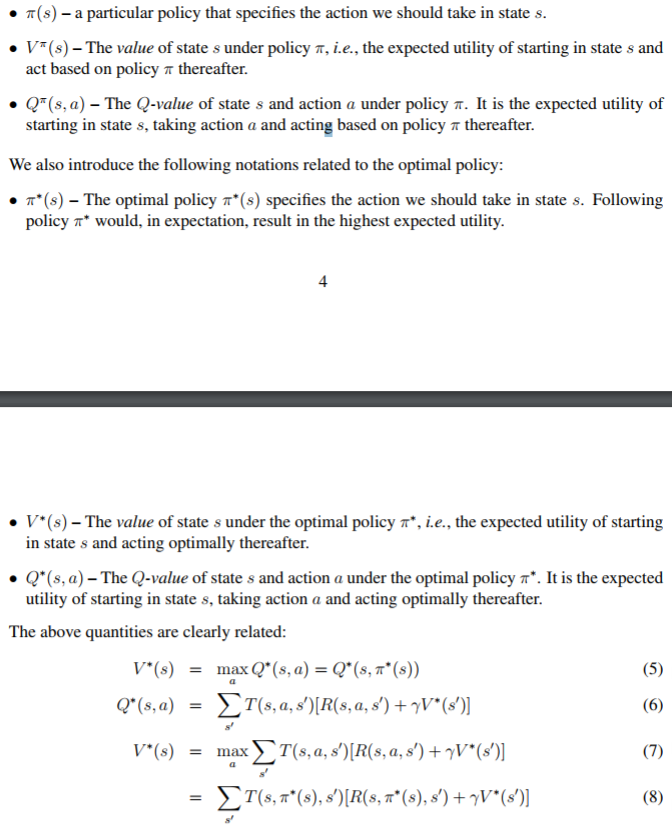
\includegraphics{D:/Documents/projects/201709.university.t6/assets/201712150748.PNG}
\caption{model}
\end{figure}

\hypertarget{value-iteration-algorithm}{%
\subsection{Value Iteration algorithm}\label{value-iteration-algorithm}}

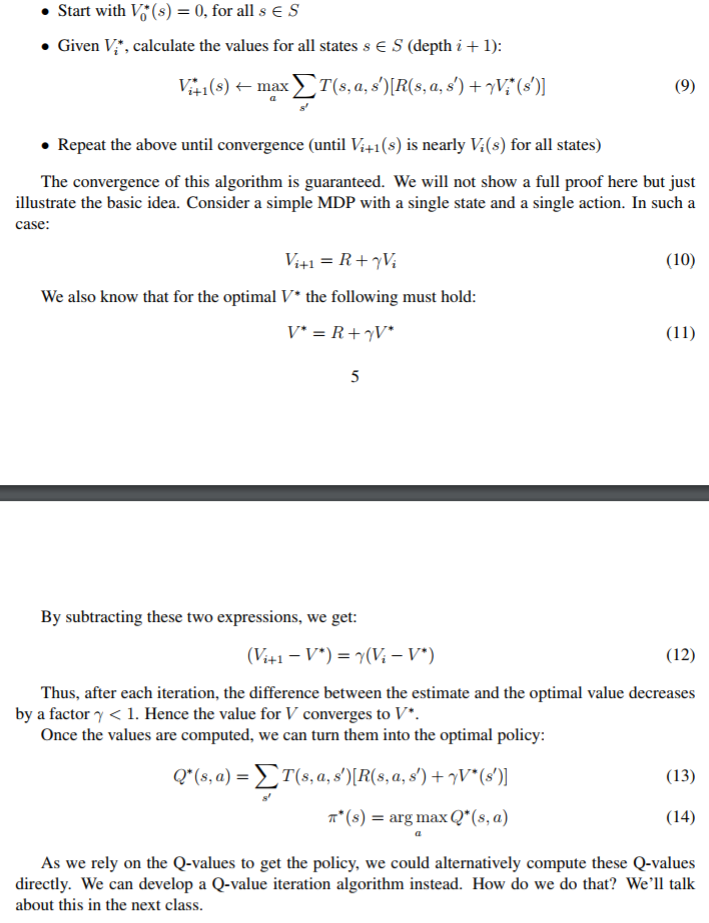
\includegraphics{D:/Documents/projects/201709.university.t6/assets/201712150751.PNG}

\hypertarget{q-value-iteration-algorithm}{%
\subsection{Q-Value Iteration
Algorithm}\label{q-value-iteration-algorithm}}

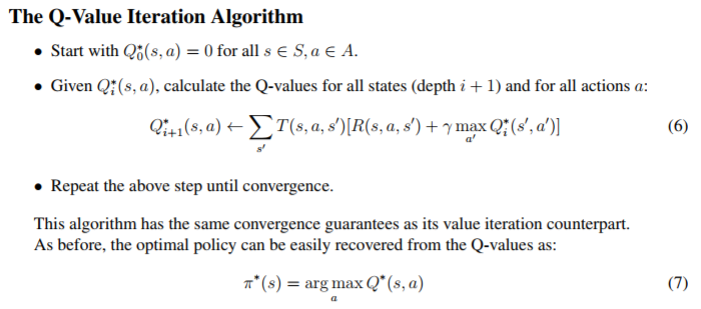
\includegraphics{D:/Documents/projects/201709.university.t6/assets/201712150752.PNG}

\hypertarget{q-learning-algorithm}{%
\subsection{Q Learning Algorithm}\label{q-learning-algorithm}}

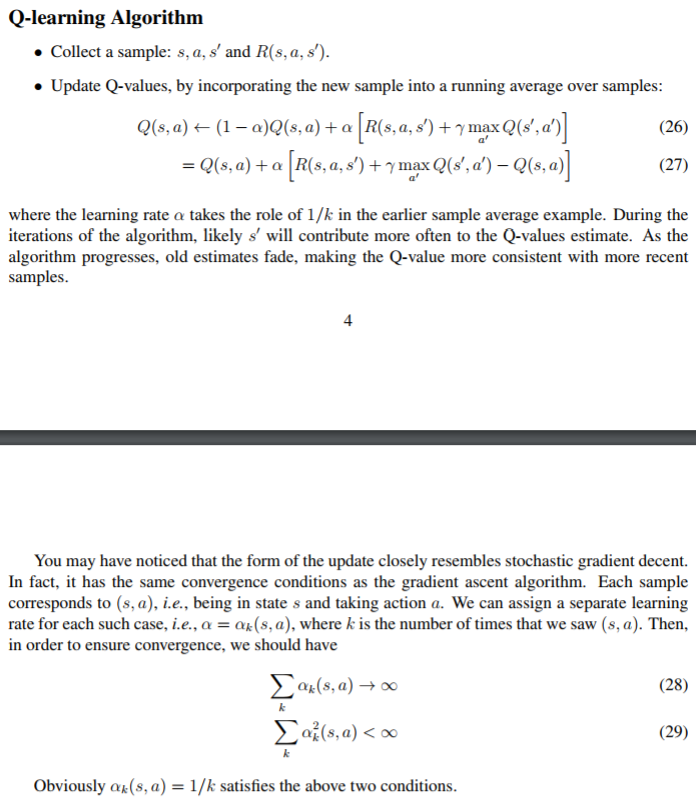
\includegraphics{D:/Documents/projects/201709.university.t6/assets/201712150754.PNG}


    % Add a bibliography block to the postdoc
    
    
    
    \end{document}
